% arara: pdflatex: { synctex: yes }
% arara: makeindex: { style: ctuthesis }
% arara: bibtex

% The class takes all the key=value arguments that \ctusetup does,
% and a couple more: draft and oneside
\documentclass[twoside]{ctuthesis}

\ctusetup{
	% preprint = \today,
	mainlanguage = english,
	otherlanguages = {czech},
	title-czech = {Gamifikace ve výuce anglických slovíček},
	title-english = {Gamification for English Vocabulary Learning},
	subtitle-czech = {},
	subtitle-english = {},
	doctype = B,
	faculty = F3,
	department-czech = {Katedra počítačové grafiky a interakce},
	department-english = {Department of Computer Graphics and Interaction},
	author = {Petr Nejedlý},
	supervisor = {Ing. Ivo Malý, Ph.D.},
	% supervisor-address = {KN:E-425, \\ Karlovo náměstí 13, \\ Praha 2},
	fieldofstudy-english = {Software Engineering and Technology},
	subfieldofstudy-english = {Business informatics},
	fieldofstudy-czech = {Softwarové inženýrství a technologie},
	subfieldofstudy-czech = {Business informatics},
	keywords-czech = {gamifikace, anglická slovíčka, mobilní aplikace, Flutter},
	keywords-english = {gamification, English vocabulary, mobile app, Flutter},
	day = 5,
	month = 1,
	year = 2025
%	specification-file = {ctutest-zadani.pdf},
%	front-specification = true,
%	front-list-of-figures = false,
%	front-list-of-tables = false,
%	monochrome = true,
%	layout-short = true,
}

\ctuprocess

\setlength{\parskip}{1em}

\addto\ctucaptionsczech{%
	\def\supervisorname{Vedoucí}%
	\def\subfieldofstudyname{Studijní program}%
}

\ctutemplateset{maketitle twocolumn default}{
	\begin{twocolumnfrontmatterpage}
		\ctutemplate{twocolumn.thanks}
		\ctutemplate{twocolumn.declaration}
		\ctutemplate{twocolumn.abstract.in.titlelanguage}
		\ctutemplate{twocolumn.abstract.in.secondlanguage}
		\ctutemplate{twocolumn.tableofcontents}
		\ctutemplate{twocolumn.listoffigures}
	\end{twocolumnfrontmatterpage}
}

% ----- Abstract -----
\begin{abstract-czech}
TODO: tady bude abstrakt v češtině
\end{abstract-czech}

\begin{abstract-english}
TODO: here will be an abstract in English
\end{abstract-english}

% ----- Acknowledgements -----
\begin{thanks}
TODO: Acknowledgements...
\end{thanks}

% ----- Declaration -----
\begin{declaration}
TODO: Declaration...

In Prague,~\monthinlanguage{title} \ctufield{day},~\ctufield{year}
\end{declaration}

% --------------------------------------------

\begin{document}

\maketitle

% ----- THESIS TEXT (indiviual chapters) -----
\chapter{Introduction}

TODO: introduction and motivation...

\section{Objectives and Goals}

TODO: ...

\chapter{Mobile Application: English Mind}
\label{chap:mobile-application-english-mind}

English Mind is a mobile application available on Android \cite{cite:english_mind_play_store} and iOS \cite{cite:english_mind_app_store} platforms that focuses on learning English vocabulary. To achieve high efficiency in learning new English vocabulary, the application combines three main teaching methods on which it is based \cite{cite:english_mind_website}:

\begin{itemize}
    \item Frequency list of English vocabulary
    \item Active recall utilizing flashcards
    \item Spaced repetition system
\end{itemize}

These methods create a structured and efficient approach to mastering vocabulary effortlessly, setting the app apart from its competitors in the field of vocabulary learning apps.

\section{Frequency List}

Frequency list is a ranked list of words, where individual words are ordered according to their frequency of occurrence in common texts and speech. 

One possible use of frequency lists is in the area of vocabulary teaching for foreign language learners. If the student learns new vocabulary words sequentially according to a frequency list, the student will encounter the newly learned words more often outside of the learning environment and thus understand more of the foreign text and speech. Conversely, if the student were to learn vocabulary randomly, the student is more likely to learn vocabulary that is too difficult relative to his current language skills, which would reduce the effectiveness of the learning process and slow his or her progress.

The importance of teaching English vocabulary according to the frequency list is supported by the results of the study \textit{How Large a Vocabulary is Needed For Reading and Listening?} \cite{cite:nation2006_how_large_vocabulary_is_needed}. This looked at how much word-family vocabulary is needed to understand most written English text and speech. The results showed that a 1,000 word-family vocabulary is needed to understand 78-81\% of most written text and a 8,000-9,000 word-family vocabulary is needed to understand 98\% of most written text. These data show the important role that frequency lists represent in effective vocabulary acquisition. If a student learns new vocabulary according to a frequency word list, he or she will understand more of the text and conversations much sooner than if he or she learns new vocabulary randomly.

\subsection{Implementation in English Mind}

The specific implementation of the English vocabulary frequency list in the mobile application is as follows. All the vocabulary words are sorted in the app according to their frequency of occurrence in common speech and English texts. As shown in Figure~\ref{fig:em-frequency-list}, user has the possibility to browse through the ranked words and change their status. 

\begin{figure}[!h]
    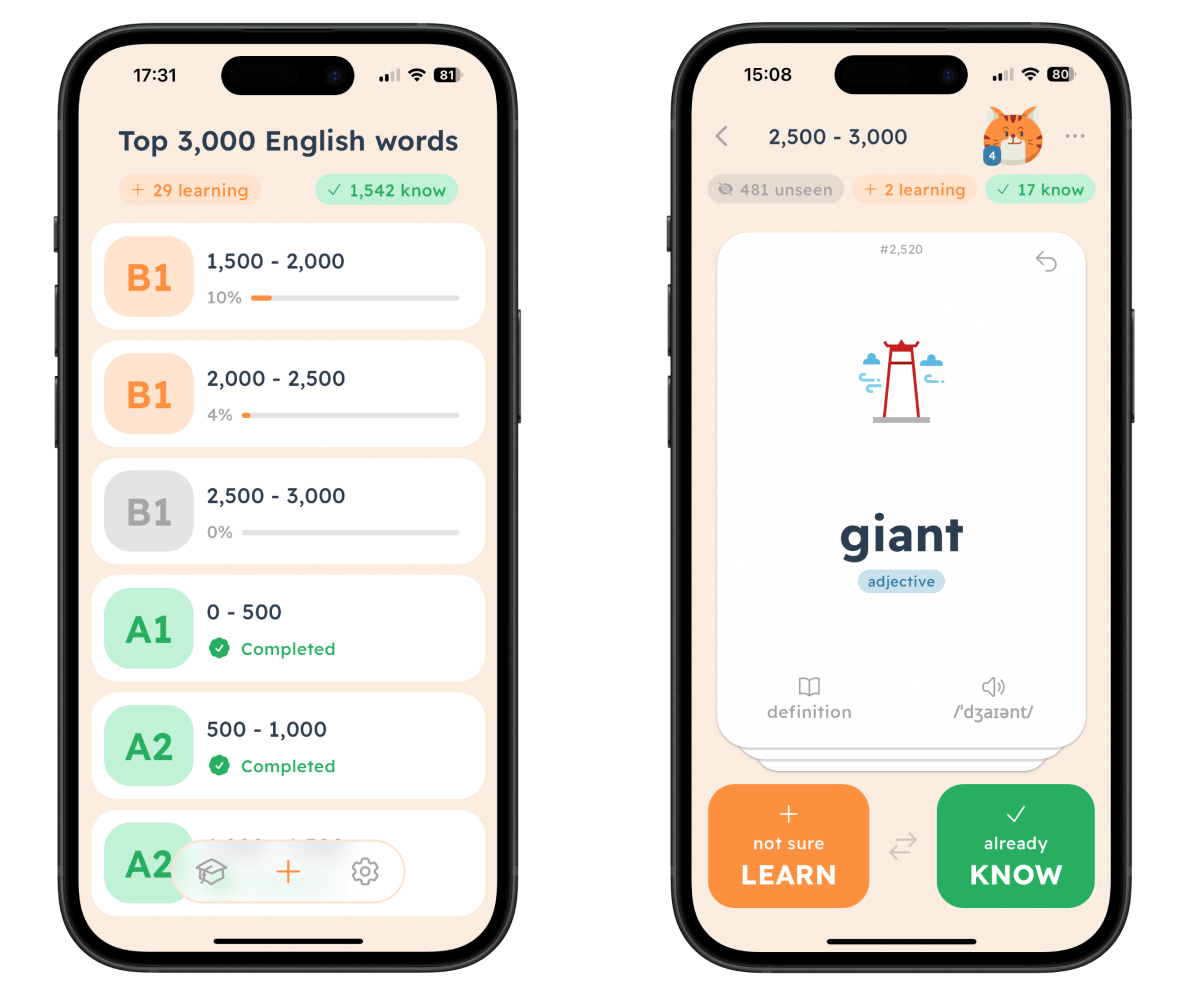
\includegraphics[width=0.65\textwidth]{chapters/images/em-frequency-list.png}
    \caption{English Mind - Implementation of a Frequency List}
    \label{fig:em-frequency-list}
\end{figure}

Each word has a status that can take three different values - unseen, know or learning. The default status value is unseen, which represents words that the user has not yet encountered in the application and has not expressed whether or not he knows the word. Words with the know status represent words that the user considers to be familiar to him and does not need to practice them. The learning status, on the other hand, represents words that the user does not know and would like to learn. These learning status vocabulary words are then practiced by the user using flashcards and the spaced repetition system method, which are discussed in later chapters.

\section{Active Recall and Flashcards}

Active recall is a method that focuses on how information is repeated during learning. The aim of the method is for the student to actively try to recall the correct answer instead of memorizing the information by rereading the correct answer (passive review). Both methods, active recall and passive review, have advantages and disadvantages. However, in the area of effective vocabulary learning, active recall seems to be preferable as it achieves better results for long-term memorization of information (in our case, vocabulary words).

This is shown in a study conducted at Washington University in 2006 \cite{cite:rhkj2006_longterm_retention}, which involved reading a text and then testing its comprehension. The text for reading comprehension was divided into 30 idea units for scoring purposes. A total of 120 students between the ages of 18 and 24 participated in the study and were divided into three groups. The groups differed in the amount of time (5 minutes, 2 days, 1 week) between reading the text and taking the assessment test. Each of the three groups was further divided into two subgroups, with the first subgroup having twice as much time to memorize and understand the text. The second subgroup had only one half of the time to read the text, but compared to the first subgroup, they had the opportunity to use the active recall method in the other half of the remaining time. The final results of the study showed that the active recall method appears to be more successful for remembering information for a longer time interval compared to the passive review method (see Figure \ref{fig:active-recall-passive-review-results}).

\begin{figure}[!h]
    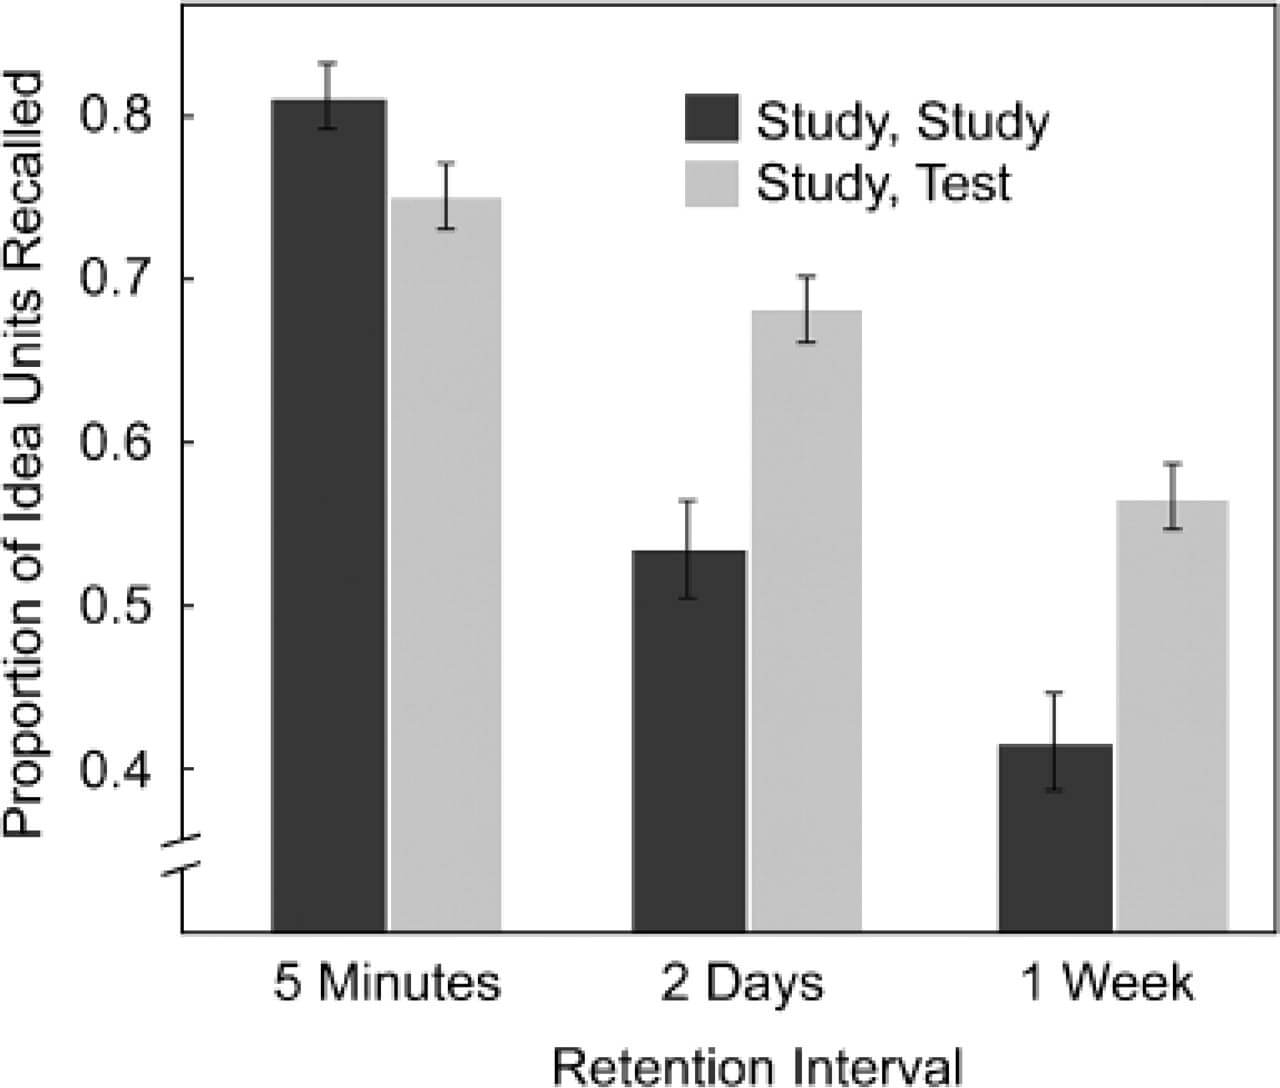
\includegraphics[width=0.6\textwidth]{chapters/images/active-recall-passive-review-results.jpeg}
    \caption{Mean proportion of idea units recalled on the final test after a 5-min, 2-day, or 1-week retention interval as a function of learning condition (passive review vs. active recall). Error bars represent standard errors of the means. \cite{cite:rhkj2006_longterm_retention}}
    \label{fig:active-recall-passive-review-results}
\end{figure}

One of the most common implementations of the active recall method is using flashcards. The principle of flashcards is based on paper cards where the student writes a question on one side and the answer on the other side. While learning, the student goes through the flashcards by first asking the question without seeing the correct answer, and after answering the question, he can immediately check the correctness of his answer by flipping the flashcard over. This gives him immediate feedback and he can easily see which questions he already knows and which he needs to repeat.

\subsection{Implementation in English Mind}

The mobile application implements the active recall method using the flashcards mentioned above. On the front side of the flashcard there is an English word and on the other side the meaning of the word in the form of a definition, sample sentences for better understanding of the use of the word, pronunciation, picture and translation into the user's native language. The user goes through the flashcards one by one and always tries to actively recall the meaning of the vocabulary and its usage before revealing the second side of the flashcard. 

\begin{figure}[!h]
    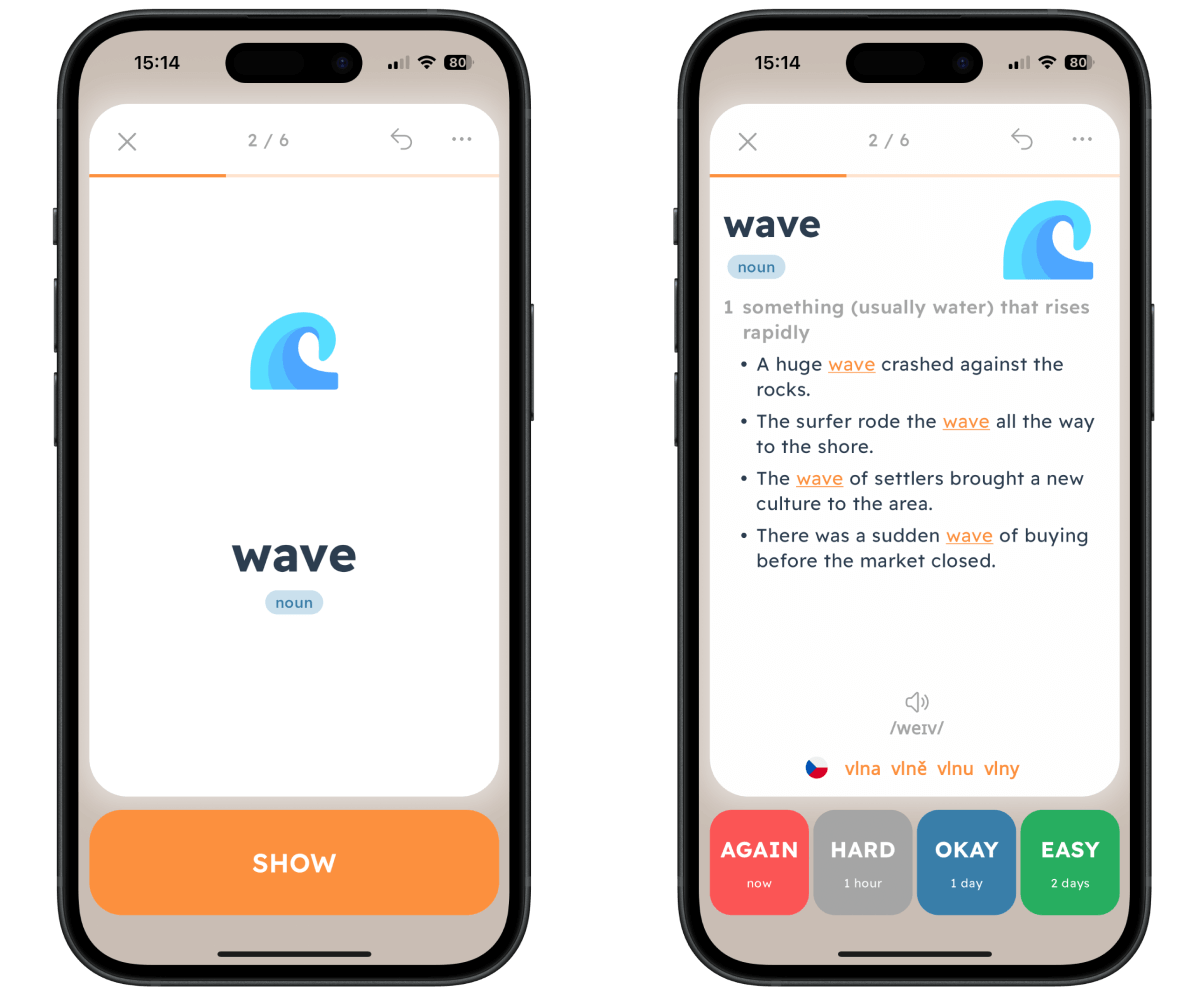
\includegraphics[width=0.65\textwidth]{chapters/images/em-flashcards.png}
    \caption{English Mind - Implementation of Active Recall Utilizing Flashcards}
    \label{fig:em-flashcards}
\end{figure}

\section{Spaced Repetition System (SRS)}

The Spaced Repetition System (SRS) is a teaching method that uses time intervals between repetitions to improve long-term retention of information. The principle of SRS is based on the theory of forgetting first formulated by German psychologist Hermann Ebbinghaus in the 19th century \cite{cite:ebbinghaus2013_memory_contribution_to_experimantal_psychology}. He found out that we forget most of the information shortly after learning it, but if the information is repeated just before we begin to forget it, it can be retained much longer.

A key aspect of SRS is adjusting the length of the intervals between repetitions based on how well the student remembers the information. Information that is easily remembered by the student is repeated less often, while information that is forgotten more quickly is repeated more often \cite{cite:kang2016_spaced_repetiton_promotes_efficient_learning}.

SRS greatly increases learning efficiency and promotes long-term retention of information by optimizing the timing of repetition based on the forgetting curve, minimizing the time spent unnecessarily repeating already well-remembered information \cite{cite:kang2016_spaced_repetiton_promotes_efficient_learning}.

\subsection{Implementation in English Mind}

Spaced repetition system is implemented in the application as follows. The user adds a word he wants to learn by changing its status to learning. The word is then displayed to the user in a queue of flashcards to practice. As the user goes through the flashcards queue, the second side of the flashcard always reveals the meaning of the vocabulary word with four SRS buttons — AGAIN, HARD, OKAY and EASY (see Figure \ref{fig:em-srs-flashcard}).

\begin{figure}[!h]
    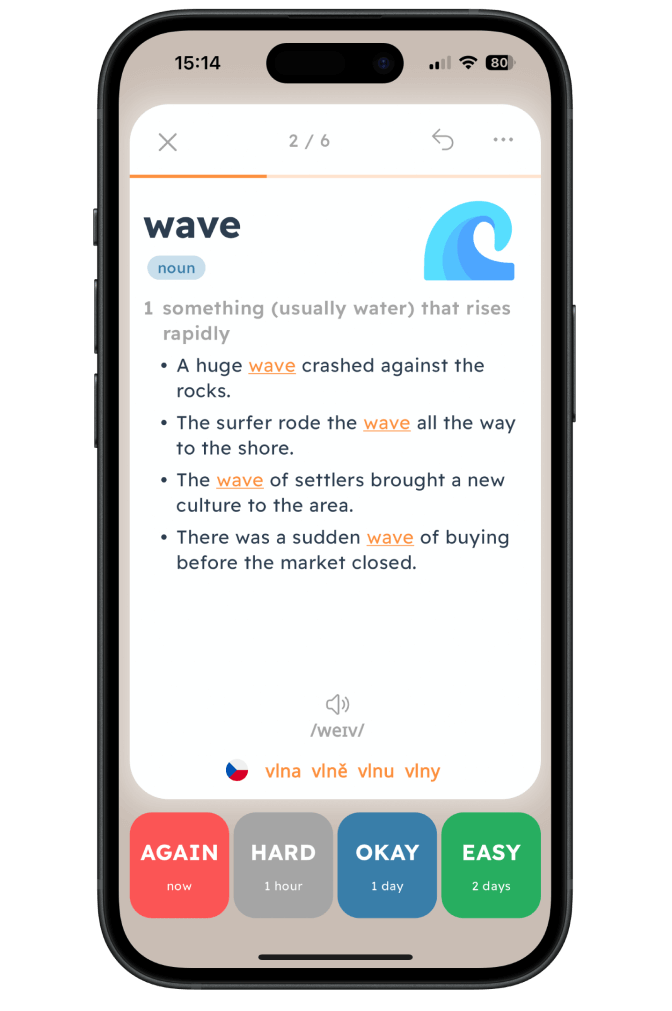
\includegraphics[width=0.42\textwidth]{chapters/images/em-srs-flashcard.png}
    \caption{English Mind - Implementation of SRS (highlighted in red)}
    \label{fig:em-srs-flashcard}
\end{figure}

Each SRS button displays information about the interval between next repeating. The AGAIN and HARD buttons shorten the interval between the next repetition, while the OKAY and EASY buttons lengthen the interval. When the selected interval has elapsed, the word will appear again in the flashcards queue for practice.

When a certain interval of several months between repetitions is reached, the vocabulary is considered to have been learned. This vocabulary will automatically change its status from learning to know and will no longer appear in the user's vocabulary queue.


\part{Analysis}
\chapter{Gamification of vocabulary learning for English Mind}

The motivation behind gamifying vocabulary learning is to increase learning efficiency and long-term retention through the inclusion of game elements that increase user motivation and engagement. Traditional methods of vocabulary learning, such as mechanical repetition or passive reading, can often be monotonous and lead to a decline in interest. Gamification brings these methods to life through elements such as rewards, challenges and competitions, leading to higher intrinsic learner's motivation.

By using gamification mechanisms it is possible to create an environment that is not only more interesting for students but also encourages repeated and focused learning. In this way, the student might remember the vocabulary better, not only on a short-term basis, but especially in the long term, which is one of the main goals of vocabulary learning.

Gamification encompasses a vast array of concepts, including streaks, badges, achievements, challenges, quests, leaderboards, rewards, statistics, progression tracking, levels and tiers, user-generated content, time-limited events, feedback loops, personalization, social elements, narrative and storytelling, virtual currencies, and so on. Furthermore, all of them can be combined and mixed in various ways. Therefore, we will focus on a selected few that can significantly enhance the user experience in the English Mind app rather than trying to cover every single gamification concept that could benefit vocabulary learning.

\textbf{TODO: add citation}

\section{Current Gamification in English Mind}

English Mind currently lacks extensive gamification features, relying instead on a few elements that can be classified as basic forms of gamification. We have identified three such elements:

\begin{itemize}
    \item \textbf{Progress Tracking of Vocabulary Acquisition} 
    \label{chap:em-progess-tracking-of-vocabulary-aquisition}
    
    Users can view essential statistics regarding their vocabulary acquisition, including the number of words they already know, the number they are currently learning, and the total remaining words to uncover. These statistics are accessible on both the vocabulary levels overview screen and on the specific vocabulary level screen.

    \begin{figure}[!h]
        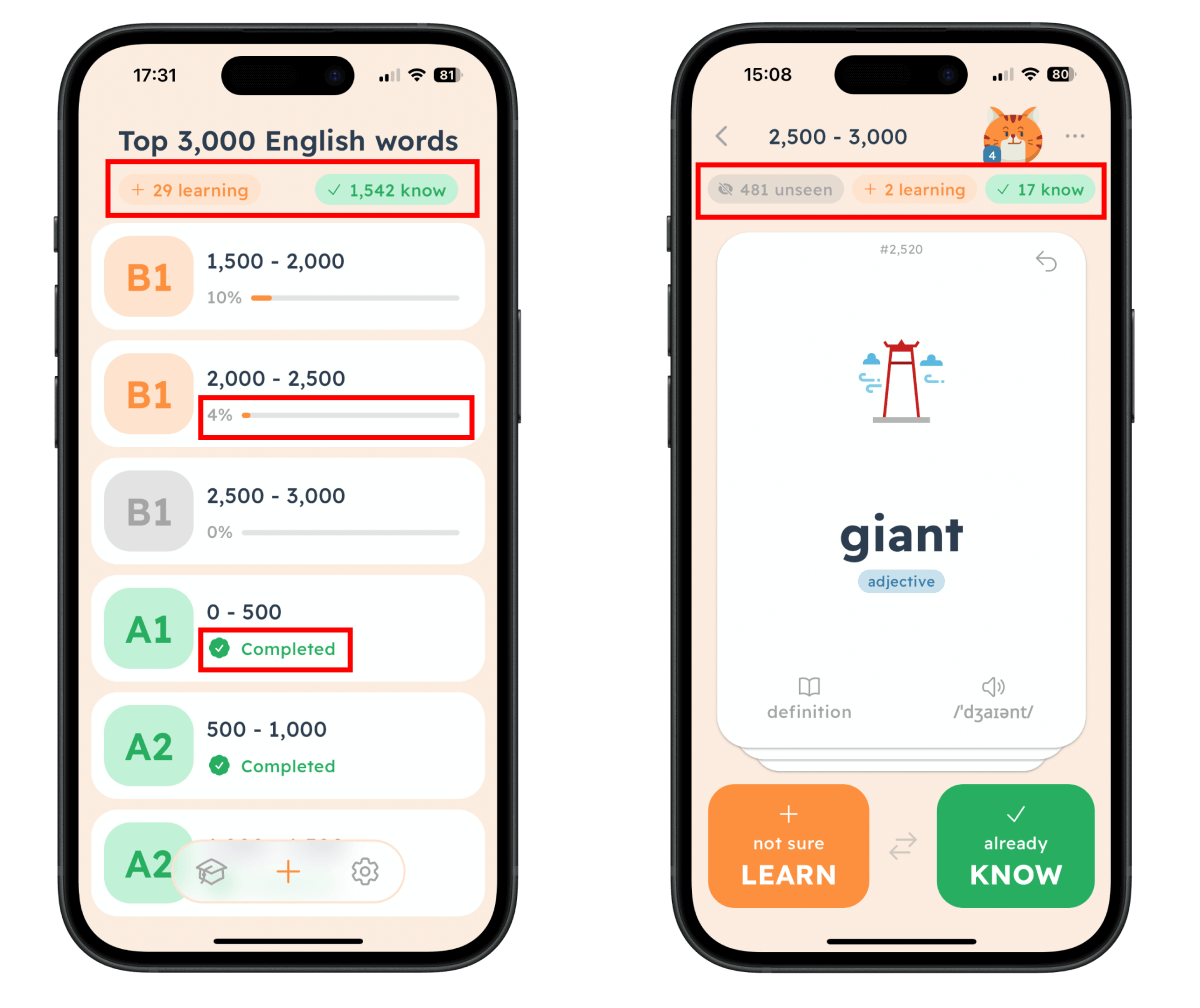
\includegraphics[width=0.65\textwidth]{chapters/images/em-progress-tracking.png}
        \caption{English Mind - Progress Tracking of Vocabulary Acquisition (highlighted in red)}
        \label{fig:em-progress-tracking}
    \end{figure}

    \item \textbf{Daily Goal}
    
    During an onboarding process, users set a personal goal for the number of new words they wish to learn or add each day.

    Additionally, a mascot appears in the top right corner on the word addition screen to count the newly added words awaiting their first practice session (see Figure \ref{fig:em-daily-goal}). This mascot serves a dual purpose, it tracks word additions and helps ensure that users do not overwhelm themselves by adding too many new words to learn at once.

    \begin{figure}[!h]
        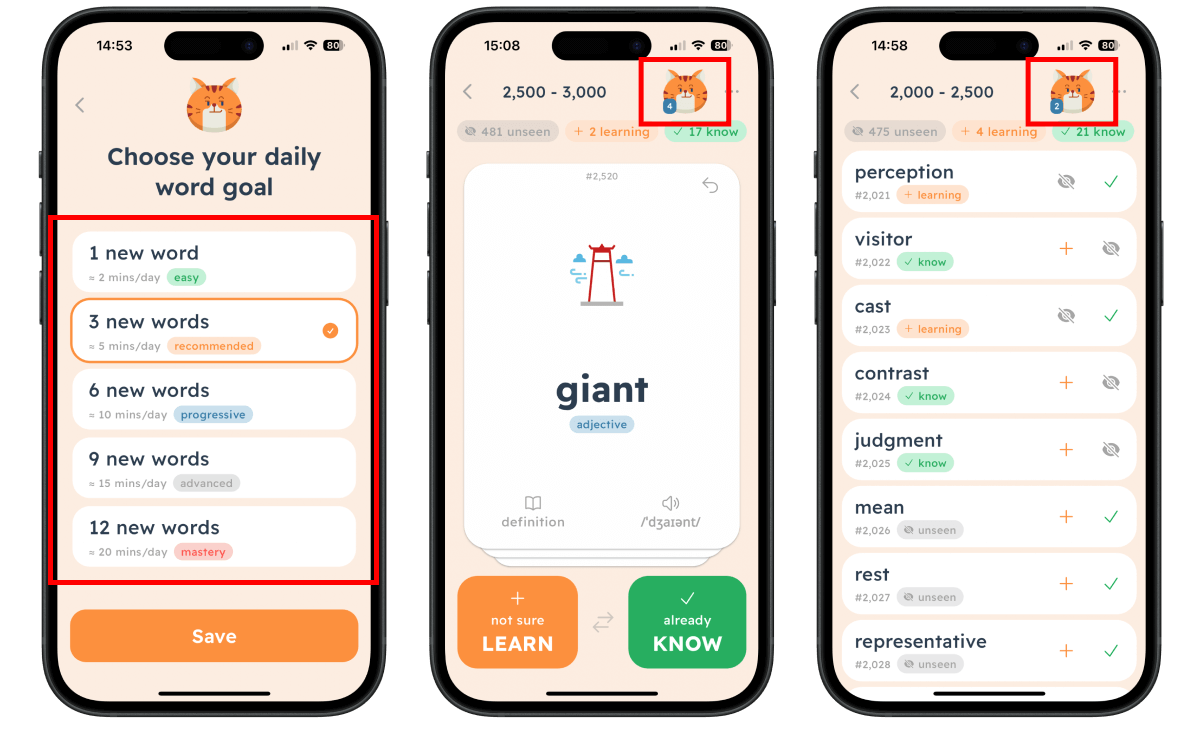
\includegraphics[width=0.8\textwidth]{chapters/images/em-daily-goal.png}
        \caption{Daily Goal and Mascot Tracking Newly Added Words to Learn (both highlighted in red)}
        \label{fig:em-daily-goal}
    \end{figure}

    \newpage

    \item \textbf{Progress Bar}
    
    While learning vocabulary through the daily queue of flashcards, users are presented with a progress bar that visually indicates their advancement, which gives them instant feedback as they progress and might motivate them to finish the current daily queue of flashcards (see Figure \ref{fig:em-flashcards-progress-bar}). Although this is a minor gamification feature, it is noteworthy given the app’s limited implementation of gamification elements.

    \begin{figure}[!h]
        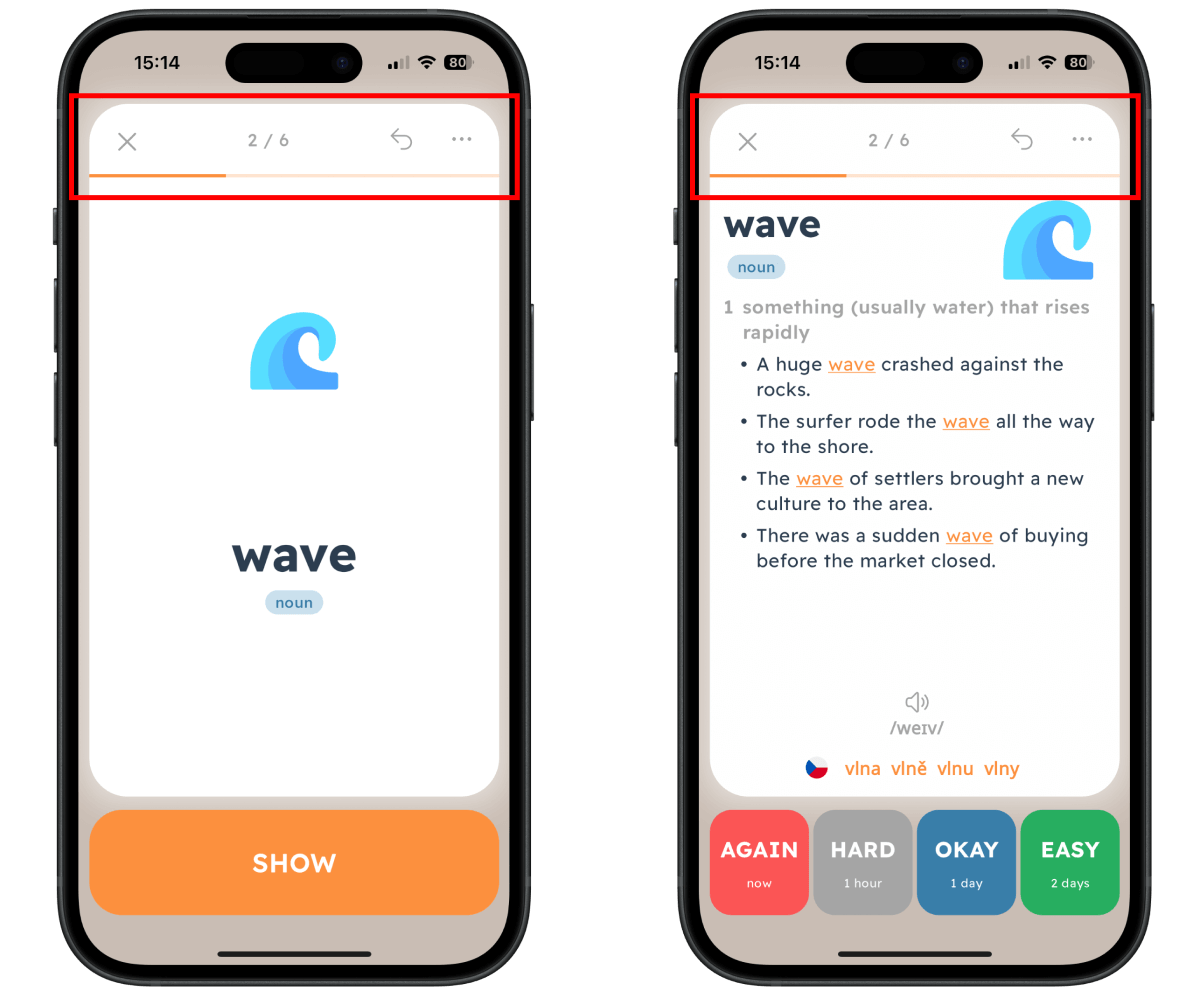
\includegraphics[width=0.65\textwidth]{chapters/images/em-flashcards-progress-bar.png}
        \caption{English Mind - Progress Bar (highlighted in red)}
        \label{fig:em-flashcards-progress-bar}
    \end{figure}
    
\end{itemize}

In summary, there is potential to enhance the app by developing a more comprehensive gamification framework, which could further enrich the user experience and encourage greater motivation for improved learning outcomes.

\section{Gamification in Similar Applications}

Before proposing new gamification features for the English Mind app, we decided to briefly analyze three mobile apps that either closely align with its learning concepts, as discussed in Chapter \ref{chap:mobile-application-english-mind}, or demonstrate innovation in the field of gamification. The selected applications are: 

\begin{itemize}
    \item \textbf{WordUp} \cite{cite:wordup}

    This app closely resembles English Mind in terms of learning concepts, as it also combines flashcards with frequency lists and a spaced repetition system.

    \item \textbf{DuoCards} \cite{cite:duocards}

    DuoCards is similar to English Mind, utilizing both flashcards and a spaced repetition system, but it lacks the incorporation of frequency lists.

    \item \textbf{Duolingo} \cite{cite:duolingo}

    While Duolingo is not based on the same learning concepts as English Mind, it was chosen for its extensive use of gamification elements and its innovations in the field. These features offer valuable inspiration for potential enhancements.
    
\end{itemize}

The following subsections will briefly explore the gamification elements used in each of these apps.

\subsection{WordUp}

WordUp application is particularly relevant as it utilizes the same learning concepts as English Mind and could inspire new gamification strategies that further support and enhance these concepts. The app has over 5 million downloads on Google Play with an average rating of 4.5 stars \cite{cite:wordup_google_play}, making it one of the most downloaded apps in English language learning field.

The app's gamification analysis identified relatively fewer gamification features despite its popularity. The vast majority of the elements identified were related in some way to practicing the flashcards queue. In the area of adding new words, a single gamification element was identified. Namely, the progress completion of a particular vocabulary range, which is very similar to the \textit{progress tracking of vocabulary acquisition} \ref{chap:em-progess-tracking-of-vocabulary-aquisition} in English Mind; therefore, it will not be listed.

Identified gamification elements are:

\begin{itemize}
    \item \textbf{Various Types of Flashcards}

     WordUp uses four different types of flashcards that are rotated regularly to break the stereotype of flashcard practice. Each flashcard type focuses on a different aspect of learning acquisition or its combination, such as meaning, spelling, and listening. This approach effectively mitigates the monotony often associated with traditional flashcard practice, thereby increasing user engagement and interest. The four types of flashcard are (see Figure \ref{fig:wordup-flashcard-types}):
    
    \begin{itemize}
        \item \textbf{Read a word and choose the correct definition}
        
        Promotes word comprehension by having users select the most accurate definition, reinforcing meaning and usage.
        
        \item \textbf{Read a definition and choose the correct word}

        Strengthens recall by prompting users to match the definition with the correct term.
        
        \item \textbf{Read a definition and choose the correct spelling}

        This type emphasizes spelling accuracy, requiring users to focus on the correct letter sequence while associating the word with its meaning.
        
        \item \textbf{Listen to a word and choose the correct spelling}

        Enhances auditory skills and spelling, as users select the correct spelling of the spoken word.
        
    \end{itemize}

    \begin{figure}[!h]
        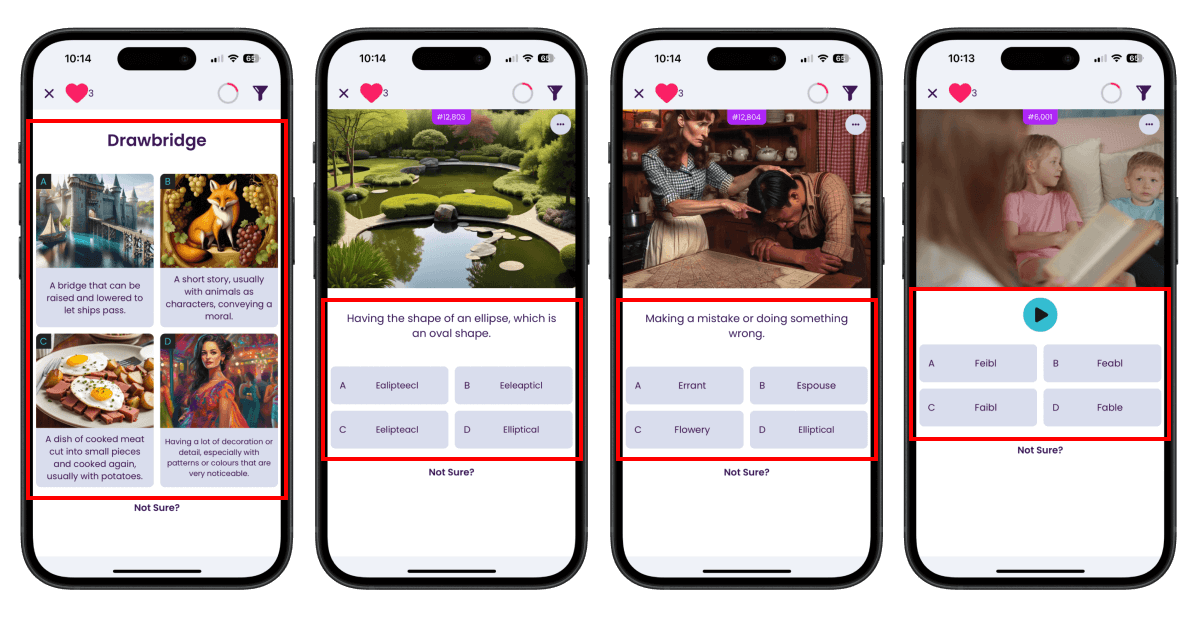
\includegraphics[width=1\textwidth]{chapters/images/wordup-flashcard-types.png}
        \caption{WordUp - Types of Flashcards (highlighted in red)}
        \label{fig:wordup-flashcard-types}
    \end{figure}
    
    \item \textbf{Progress tracking for individual words}
    
    WordUp uses its own unique spaced repetition system. It features a visual indicator that tracks each word's progress, showing how many times the user has correctly recalled it (see Figure \ref{fig:wordup-word-progress}). This interactive feedback motivates continued practice, rewarding users with a sense of achievement as they advance.

    \begin{figure}[!h]
        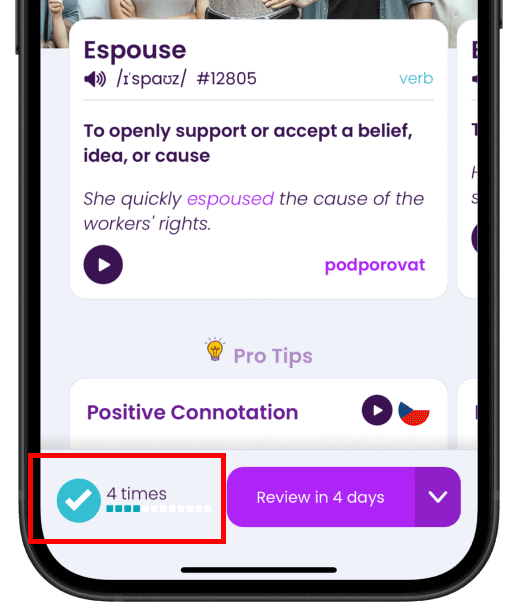
\includegraphics[width=0.35\textwidth]{chapters/images/wordup-word-progress.png}
        \caption{WordUp - Indicator of Word's Progress (highlighted in red)}
        \label{fig:wordup-word-progress}
    \end{figure}

    \item \textbf{Daily Goal and Leaderboard}

    WordUp introduces a daily goal based on minutes spent practicing to motivate users to practice regularly. First, the user sets a daily commitment for how many minutes they intend to practice English vocabulary. Each day, they strive to complete a circular progress ring representing this goal, providing a clear sense of accomplishment (see Figure \ref{fig:wordup-daily-goal}).
    
    Additionally, WordUp includes a leaderboard that ranks users based on the minutes they spend practicing (see Figure \ref{fig:wordup-daily-goal}). Users can compare their achievements with friends or other learners, adding a social and competitive element that encourages continued practice. 

    \begin{figure}[!h]
        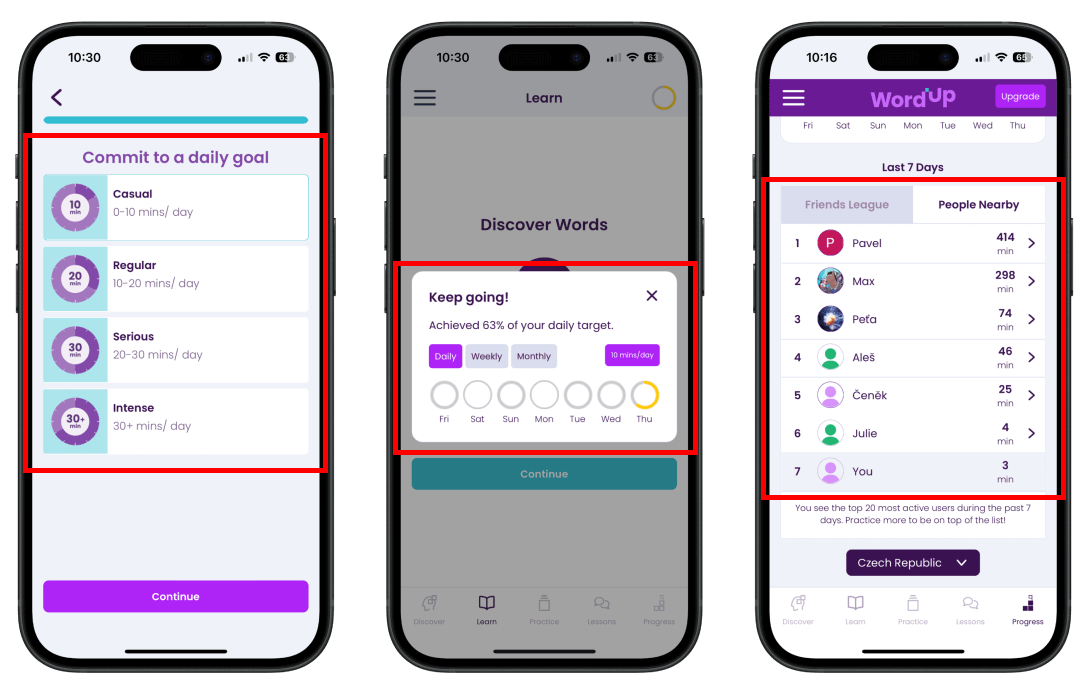
\includegraphics[width=0.99\textwidth]{chapters/images/wordup-daily-goal.png}
        \caption{WordUp - Daily Goal and Leaderboard (both highlighted in red)}
        \label{fig:wordup-daily-goal}
    \end{figure}

\end{itemize}

\subsection{DuoCards}

The DuoCards application uses an SRS-based flashcard approach for vocabulary practice and has over a million downloads on Google Play with an average rating of 4.6 stars \cite{cite:duocards_google_play}. 

The analysis of gamification features reveals two key concepts: various types of flashcards and a more complex mascot upgrade system using virtual currency. The following sections provide detailed descriptions of these two concepts.

\begin{itemize}
    \item \textbf{Various Types of Flashcards}

    Duocards utilizes four different types of flashcards (see Figure \ref{fig:duocards-flashcard-types}) to keep practice exciting and address various aspects of language acquisition, such as spelling and meaning. This gamified approach maintains user interest, enhancing the learning experience. Identified flashcard variants are:

    \begin{itemize} 
         \item \textbf{English to Native Language}
         
         Displays an English word on the front, with its translation on the back. 

         \item \textbf{Native Language to English}
         
         Reverses the direction, showing the native language word on the front and prompting the English translation on the back.
         
        \item \textbf{Pronunciation Focus}
        
        Emphasizes auditory learning by presenting only the word’s pronunciation, with spelling revealed upon flipping the flashcard. 
        
        \item \textbf{Matching Exercise}
        
        Appears periodically, involving the matching of five words with their correct translations. 
    
    \end{itemize}

    \begin{figure}[!h]
        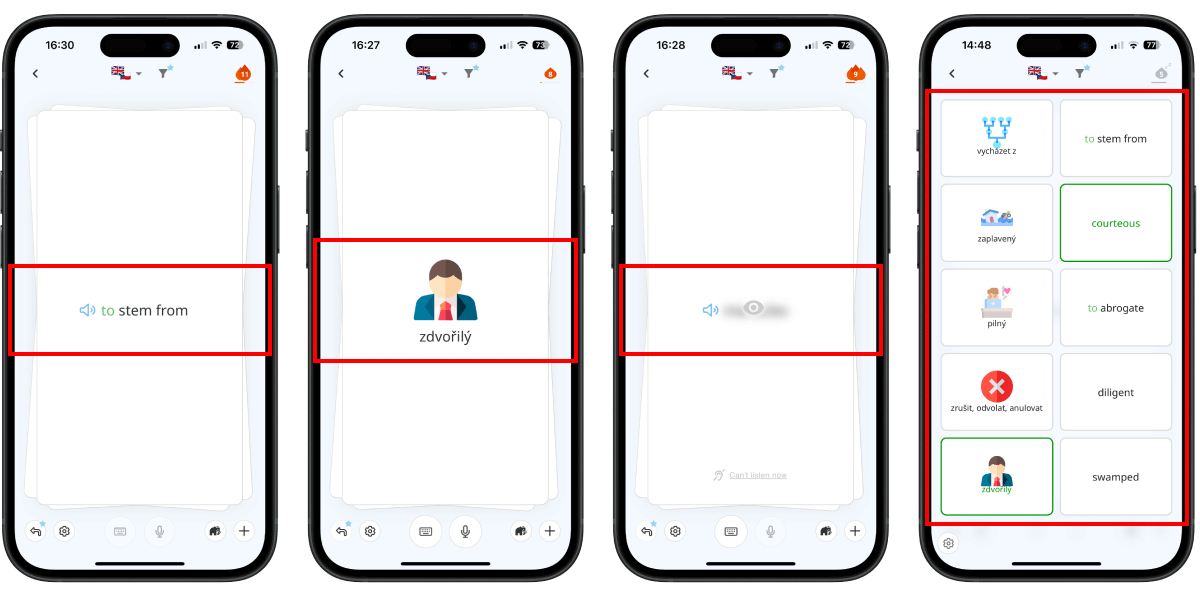
\includegraphics[width=0.98\textwidth]{chapters/images/duocards-flashcard-types.png}
        \caption{DuoCards - Types of Flashcards (highlighted in red)}
        \label{fig:duocards-flashcard-types}
    \end{figure}
    
    \item \textbf{Mascot Upgrade System and Virtual Currency}

    The app’s most intriguing gamification feature is its mascot, Memo, which lives in a customizable habitat on the main screen. Users can upgrade Memo’s home by purchasing and arranging various items, creating a personalized space for them. These upgrades require a virtual currency, XP (Experience Points), which users earn by practicing and adding new vocabulary. This system rewards learning progress and adds a creative, interactive layer to vocabulary practice.

    By engaging users in developing Memo’s habitat, the app stimulates a sense of ownership and investment in the learning process. This connection can enhance motivation and commitment to vocabulary acquisition, making learning feel more like a game than a chore. 

    \begin{figure}[!h]
        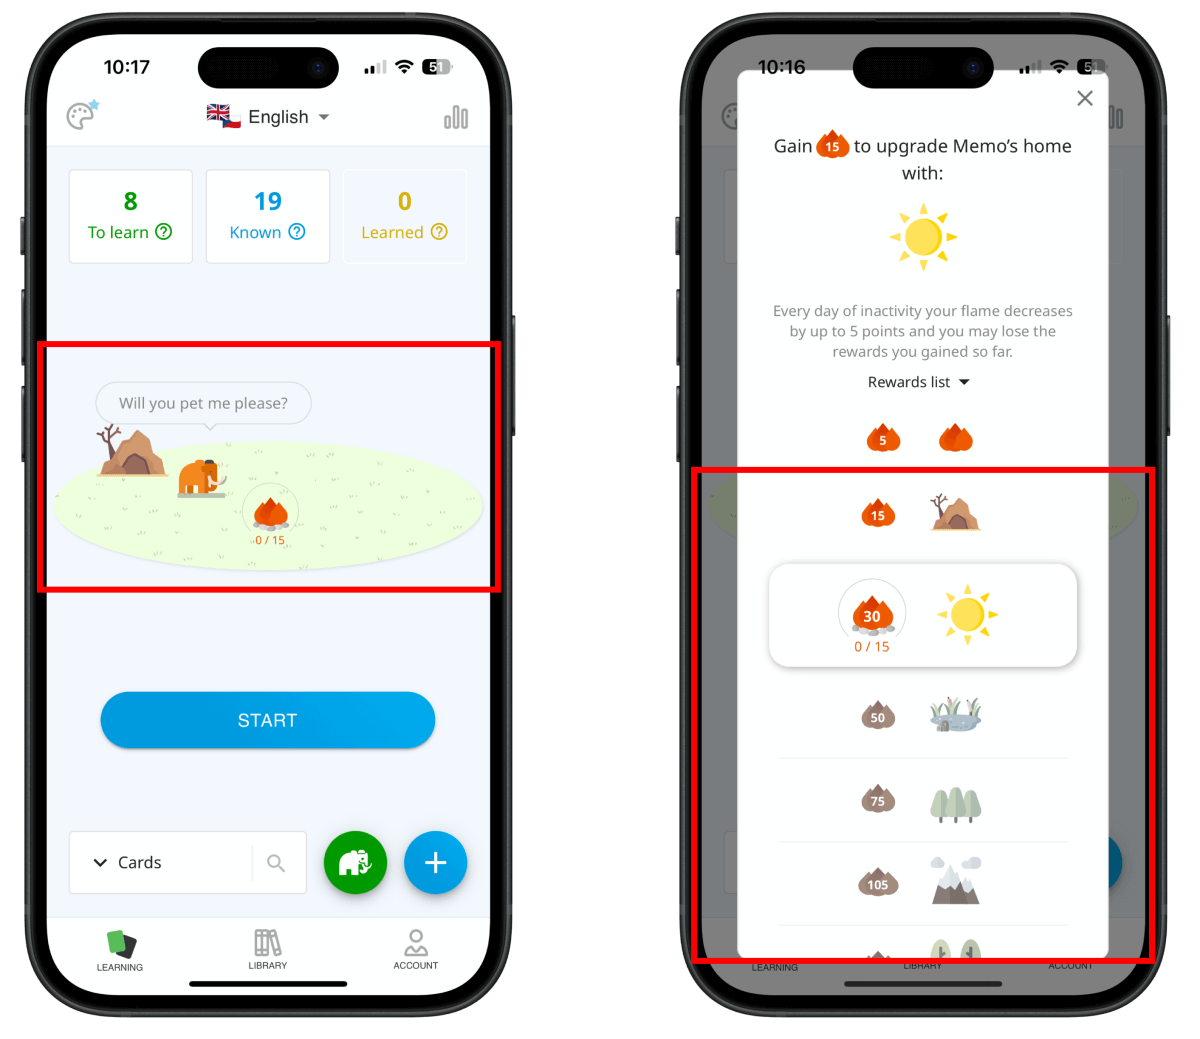
\includegraphics[width=0.8\textwidth]{chapters/images/duocards-memo.png}
        \caption{DuoCards - Mascot Upgrade System (highlighted in red)}
        \label{fig:duocards-memo}
    \end{figure}

\end{itemize}

\subsection{Duolingo}

Duolingo, the world's most popular language learning application with over 100 million monthly active users \cite{cite:duolingo_2024q2}, has revolutionized digital language education through its accessible and engaging approach. The application was chosen for analysis due to its pioneering innovations in gamification. While numerous studies have examined Duolingo's gamification strategies, we will focus only on a few elements that could be effectively adapted for English Mind, particularly those that complement its learning concepts and methodologies.

Analysis revealed three concepts that English Mind could benefit from if implemented effectively. The following sections provide a brief introduction to these concepts.

\begin{itemize}
    \item \textbf{Various Exercises}

    Duolingo structures its content into bite-sized lessons, each consisting of a series of varied exercises similar to interactive flashcards. The variety of exercises keeps users engaged as they practice. Some of these exercises include:

    \begin{itemize}
        \item \textbf{Matching pairs}

        In this exercise, users are presented with a set of five words and their translations, which they must correctly pair together (see Figure \ref{fig:duolingo-exercise-types}). This matching activity typically appears at regular intervals throughout lessons or after the introduction of new vocabulary. The interactive nature of the exercise makes vocabulary practice more engaging than traditional memorization methods.
        
        \item \textbf{Speaking practice}

        Users are presented with a sentence to pronounce, and Duolingo's speech recognition system automatically evaluates their attempts (see Figure \ref{fig:duolingo-exercise-types}). This speaking practice feature is particularly noteworthy, as many applications traditionally avoid incorporating speech exercises due to the technical challenges of natural language processing. However, with recent advancements in Large Language Models (LLMs) and their increasing accessibility, the integration of speech exercises is becoming more feasible.
        
        \item \textbf{Spelling practice}

        Users are presented with an audio recording of a sentence and must transcribe it accurately, focusing on proper spelling of each word. This exercise reinforces both listening comprehension and spelling skills (see Figure \ref{fig:duolingo-exercise-types}).
    \end{itemize}

    \begin{figure}[!h]
        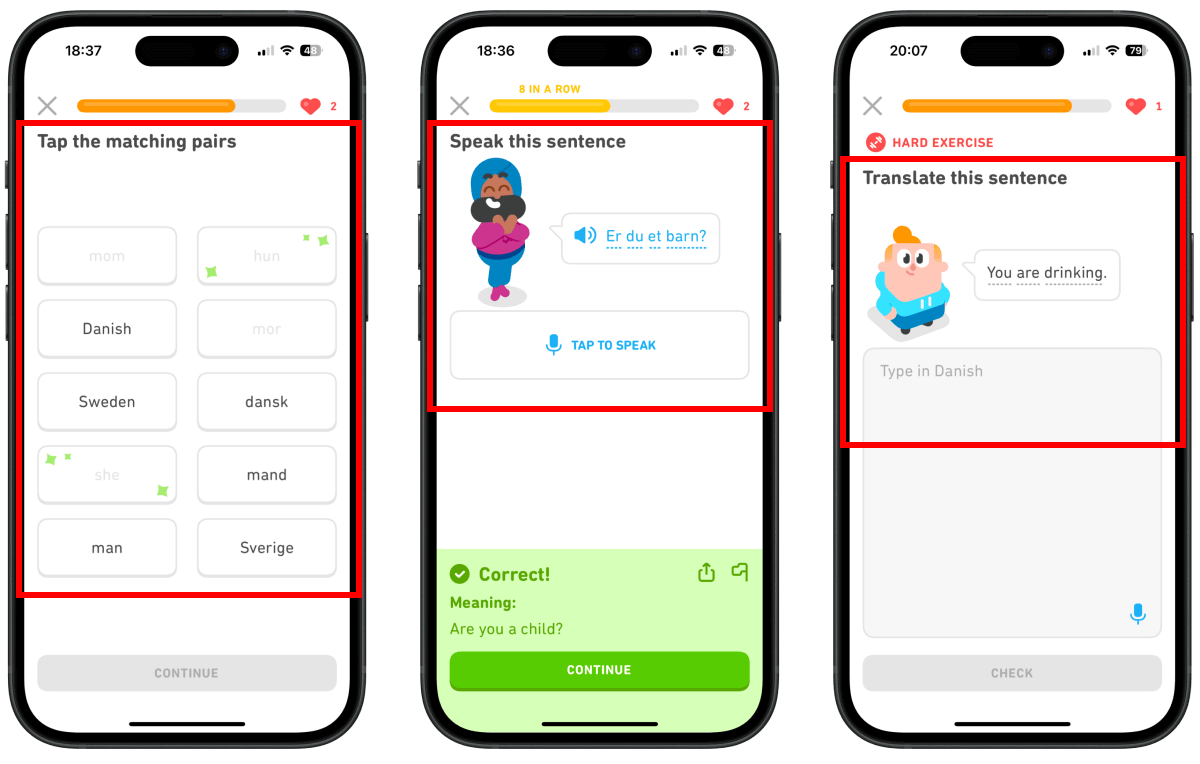
\includegraphics[width=1\textwidth]{chapters/images/duolingo-exercise-types.png}
        \caption{Duolingo - Types of Exercises (highlighted in red)}
        \label{fig:duolingo-exercise-types}
    \end{figure}

    \item \textbf{Short Review After Finishing a Lesson}

    After completing each lesson, Duolingo presents users with an engaging summary screen accompanied by a celebratory animation (see Figure \ref{fig:duolingo-lesson-review}). The summary includes key metrics such as:

    \begin{itemize}
        \item Experience points (XP) earned
        \item Accuracy rate for the completed exercises
        \item Time spent practicing
        \item Maintenance of learning streaks
    \end{itemize}

    This immediate feedback loop is crucial for user motivation, as it provides a sense of achievement and progress tracking. The inclusion of XP points and streaks transforms the learning process into a game-like experience, encouraging users to maintain consistent practice habits. The celebratory animations and positive reinforcement help create a rewarding atmosphere, making the learning process more enjoyable.

    \begin{figure}[!h]
        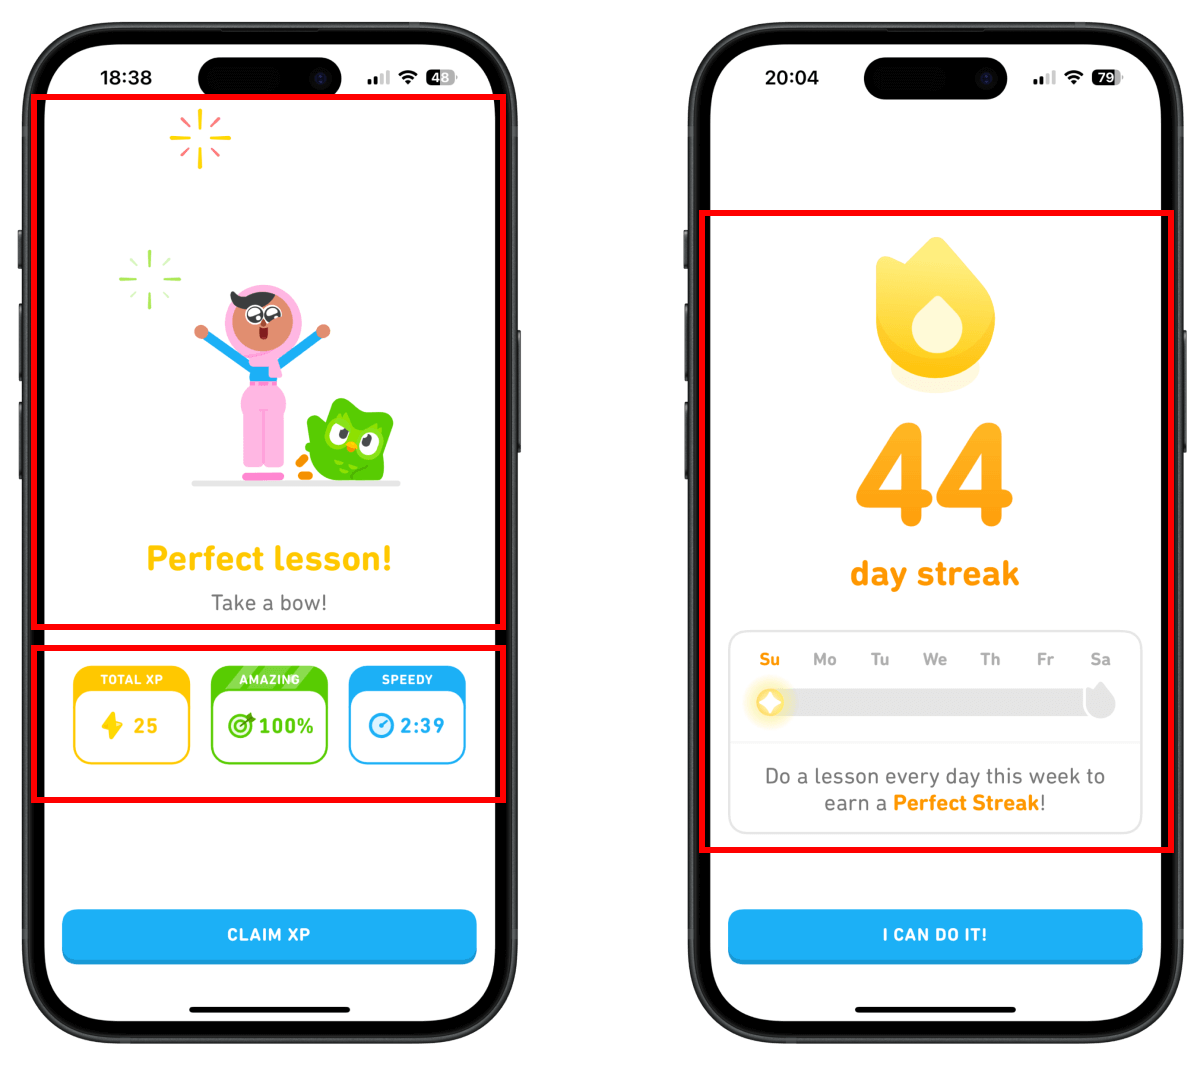
\includegraphics[width=1\textwidth]{chapters/images/duolingo-lesson-review.png}
        \caption{Duolingo - Review After Finishing a Lesson (highlighted in red)}
        \label{fig:duolingo-lesson-review}
    \end{figure}

    \item \textbf{Daily Streak}

    One of Duolingo's most powerful gamification features is the daily streak system, which tracks consecutive days of learning activity (see Figure \ref{fig:duolingo-daily-streak}). Users maintain their streak by completing at least one lesson each day, creating a powerful psychological incentive for consistent practice. To make this system more flexible and user-friendly, Duolingo introduced "Streak Freezes" - items that users can acquire to preserve their streak during a day of inactivity.

    The streak system is supported by a sophisticated notification framework that employs various psychological triggers to maintain user engagement. These include:

    \begin{itemize}
        \item Reminder notifications at user-specified times
        \item Warnings when streaks are at risk of breaking
        \item Motivational messages to encourage streak continuation
        \item Interactive home screen widgets displaying streak counts
        \item Celebrations of streak milestones
        \item Collectible app icons that unlock at different streak milestones
    \end{itemize}

    These features work together to create multiple touchpoints throughout the user's day, combining immediate rewards with long-term achievement tracking. The effectiveness of this approach is evident in the data. Over 20\% of Duolingo's daily active users maintain streaks longer than one year \cite{cite:duolingo_2024q2}. The streak system exemplifies how gamification can transform a learning obligation into an engaging daily ritual, effectively addressing one of language learning's most significant challenges: maintaining a consistent practice.
    
    \begin{figure}[!h]
        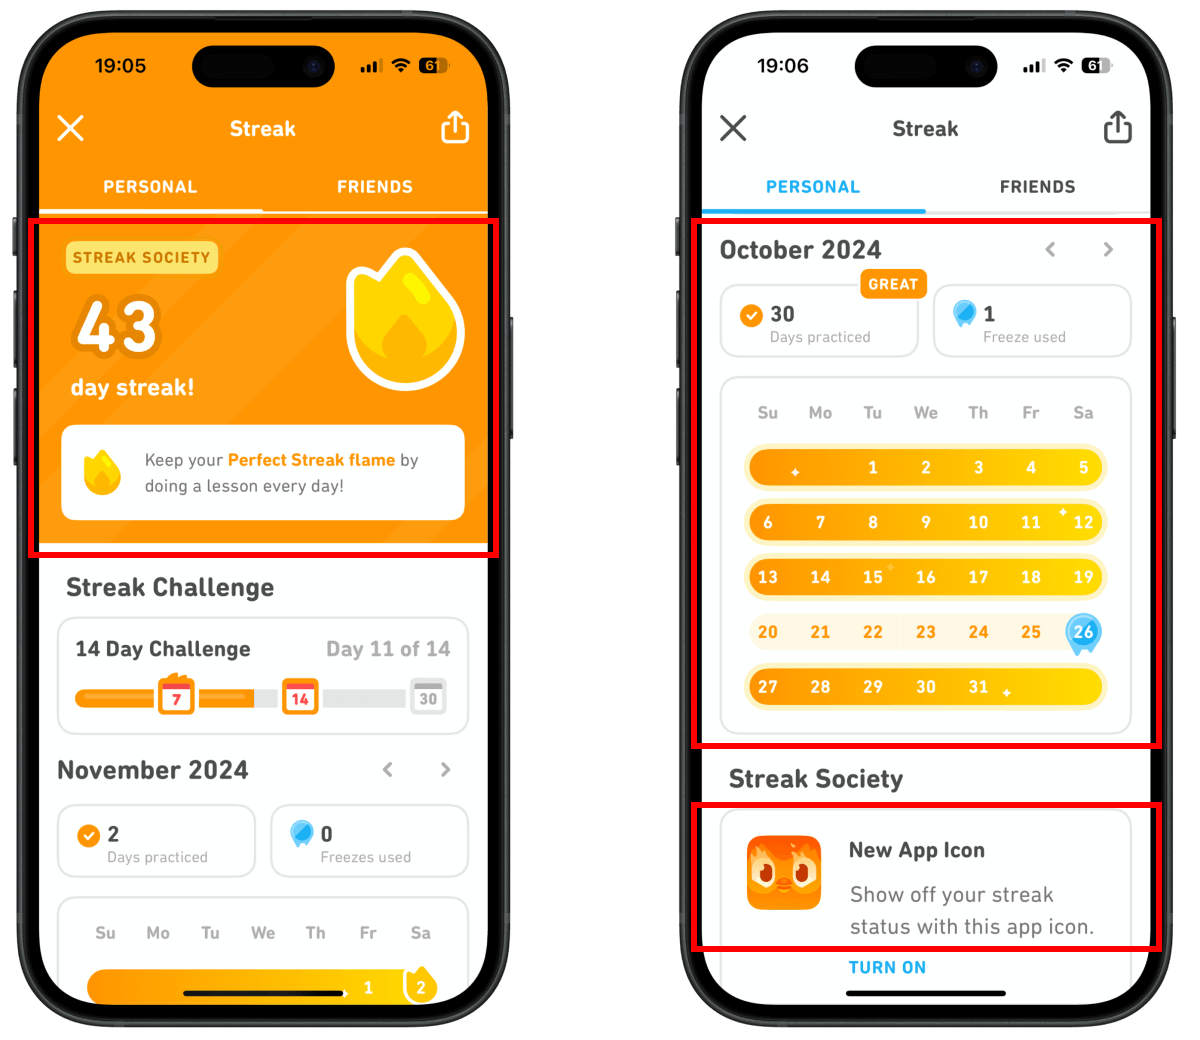
\includegraphics[width=1\textwidth]{chapters/images/duolingo-streak.png}
        \caption{Duolingo - Daily Streak (highlighted in red)}
        \label{fig:duolingo-daily-streak}
    \end{figure}
    
\end{itemize}
\chapter{Proposed Gamification Strategies and Concepts}

TODO....process behind it
what parts of the app would be the most beneficial and why to focus on them

\section{Flashcard Practice Gamification}

todo... what, why, how, desired result and benefit,...


\subsection{Flashcard Variations}

todo...

\subsection{Progress Visualization for Individual Words}

todo...

\subsection{Review After Flashcard Practice}

todo...

\section{Gamification of Adding New Words}

todo... why,...

\subsection{Daily Word Goal Visualization}

todo...

\subsection{Streak Tracking for Daily Goal}

todo...

\subsection{Quests and Word Categorization}

todo...

\section{Minigames}

todo...



\chapter{User Testing of Proposed Gamification Elements}

todo...

\section{Evaluation of Results}

todo...

\part{Implementation}
\chapter{Technology selection}
\chapter{Technology selection}
\chapter{User testing}
% --------------------------------------------

\appendix
\printindex
\bibliographystyle{unsrt}
\bibliography{chapters/bibliography}

\end{document}
